\chapter{methodisches Vorgehen}

%- Grundlagen sind notwendig zur Bewertung der Systeme
%- die exakte Definition der Anforderungen und des Ist-Standes ist Voraussetzung zur Bewertung
%- die Struktur der Untersuchung der systeme dient dem einheitlichen vergleich und der Nachvollziehbarkeit
%- konkret: aufbau ist wichtig  zur beurteilung der leistungsfähigkeit; Installation und Schnittstelle sollen aufzeigen, dass das system unter der definierten Umgebung lauffähig ist; Datenimport zeigt die integrationsfähigkeit; Verarbeitung als wesentlicher Punkt, neben Aufbau Voraussetzung für Leistung, ; Leistungstests als quelle zum Vergleich der leistung
%- Verweis auf bestehende vergleiche (literatur)

%Dan:
%du wirst bestimmt dinge finden wie "Benchmark von Datenbanken"
% und ich meine ein gis ist ja nur eine DB (mit effizienter Datenhaltung für geographische Figuren) mit erweiterten Funktionen im gis kontext
%zu bewertung von software/is würde ich auf softwaretechnik bücher verweisen ... die du verwenden kannst, um dir eine eigene Liste von  Bewertungskritierien für deinen Anwendungsfall zu erstellen

Das Thema "Untersuchung und Optimierung von verteilten geografischen Informationssystemen zur Verarbeitung agrartechnischer Kennzahlen" besteht aus vier Unteraufgaben:\\

\textbf{Untersuchung bestehender Frameworks anhand von Qualitätsmerkmalen}\\
Die erste Hälfte dieser Arbeit ist eine Softwareauswahl im Bereich der Datenverarbeitung.
Es handelt sich dabei nicht um Anwendersoftware, wodurch keine empirischen Studien der Benutzung der Frameworks durch Anwender und keine Kopplung mit der Unternehmensstruktur notwendig ist.
In diesem speziellen technischen Kontext sind wissenschaftliche Vorgehensweisen zur Softwareauswahl notwendig.
Darin soll mit Mitteln des Softwarequalitätsmanagement und allgemein Prinzipien der Softwareentwicklung eine nachvollziehbare, auch auf ähnliche Projekte übertragbare und wissenschaftlich korrekte Vorgehensweise erreicht werden.
Dafür geeignet ist eine Nutzwertanalyse.\\
Aus gegebenen Anforderungen\footnote{siehe \ref{Anforderungen}} sind Qualitätsmerkmale zu erstellen.
Davon ist die Mindestmenge welche zur Eignung eines Frameworks notwendig ist bzw. die notwendige  Qualität zu definieren.
Darauf aufbauend sind Qualitätsmetriken zu erstellen, welche die einzelnen Qualitäten messbar machen.
Eine Menge von scheinbar geeigneten Frameworks ist anhand der definierten Metriken zu untersuchen.
%TODO: auf Listen der Community zurückgreifen
Dabei sind jedoch nur die für den Anwendungsfall relevanten Qualitäten zu untersuchen.
Aus bekannten GIS Frameworks werden vielversprechende ausgewählt und somit die Menge der zu untersuchenden Frameworks erstellt.
\label{aufrufe-spatialdatabases}
Diese Vorauswahl erfolgt anhand der Tabelle \glqq Table of free systems especially for spatial data processing\grqq\ in \cite{website:wiki-spatialdatabase}.
Nicht einheitlich messbare Kriterien zur Softwareauswahl wie Marktposition, Support und Community fließen in diese Bewertung nicht ein, werden jedoch im Sinne der Agri~Con ergänzend festgehalten.

Wikpedia dient zur Vorauswahl der Frameworks als Quelle, da diese Website von Arbeitnehmern genutzt wird und somit diese Community die Tabelle aktuell und ausreichend vollständig hält.
Der Unternehmensbezug ist in der Aufrufstatistik begründet, welche in Abbildung \ref{fig:wiki-usage-spatialdatabase} dargestellt ist.
\begin{figure}
\centering
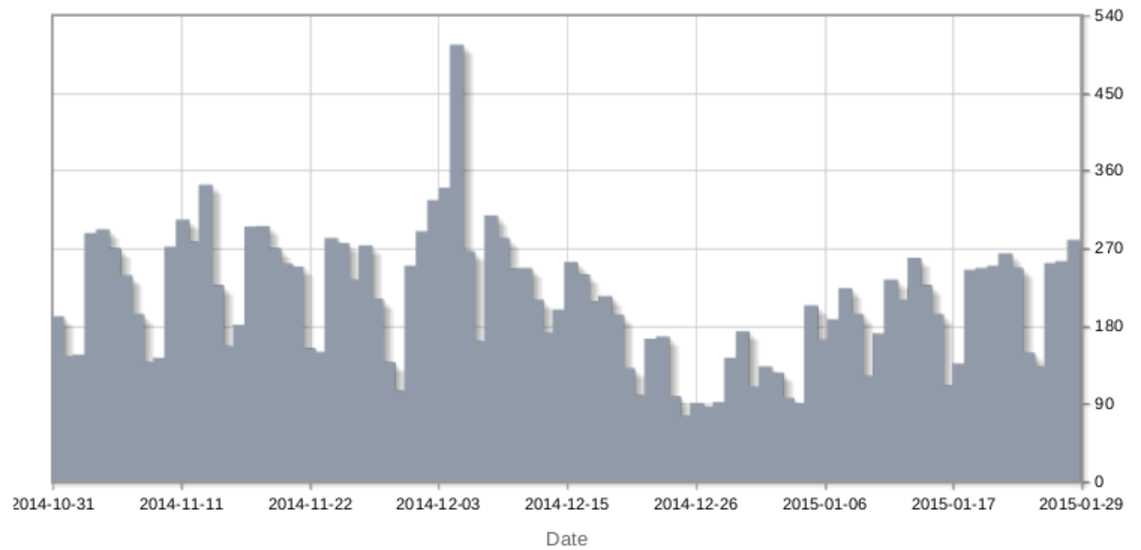
\includegraphics[width=\textwidth]{Abbildungen/wiki-spatialdatabase-usage.pdf}
\caption[Nutzungsstatistik der Wikipedia Seite spatial database]{Nutzungsstatistik von 90 Tagen der Wikipedia Seite \glqq Spatial database\grqq\ nach \cite{website:wiki-usage-spatialdatabase}}
\label{fig:wiki-usage-spatialdatabase}
\end{figure}
So wurde die Website am Mittwoch dem 21.1.2015 250 mal, dagegen am Samstag dem 17.1.2015 111 mal aufgerufen.
Allgemein ist an Tagen an Wochenenden etwa die Hälfte der Aufrufe pro Tag gegenüber Montag bis Freitag zu beobachten.
Weiterhin war zu den Weihnachtsfeiertagen eine w\Gls{topsis}esentlich geringere Anzahl an Aufrufen zu verzeichnen: 1650 Aufrufe zwischen dem 22.12.2014 und 4.1.2015 im Gegensatz zu 3005 Aufrufe zwischen dem 8.12.2014 und 21.12.2014.
Diese Aufrufstatistik belegt das die Nutzung der Website etwa zur Hälfte durch Arbeitnehmer erfolgt und somit für Unternehmen interessant ist.

\textbf{Auswahl eines Frameworks}\\
Aus der untersuchten Menge ist eines anhand der gemessenen Nutzwertes auszuwählen.
Der Ist-Stand\footnote{siehe \ref{IstStand}} der Agri~Con ist über Jahre hinweg durch wachsende  Anforderungen im technischen und organisatorischen Bereich entstanden.
Aus diesem Grund ist die Auswahl eines Frameworks für den gesuchten Anwendungsfall aufwendig.
Die Wahrscheinlichkeit der Eignung mehrerer Frameworks scheint daher nach der Einschätzung des Autors gering.
Diese induktive Hypothese gilt es in dieser Teilaufgabe zu belegen.
Eine detaillierte Bewertung der Frameworks anhand aller Qualitäten würde danach dazu führen, dass kein Framework geeignet erscheint.
Deshalb ist die Nutzwertanalyse zunächst anhand deren Spezifikationen durchzuführen.
Für derartige Entscheidungen kann stattdessen das Vorgehen \Gls{ahp} verwendet werden.
Dabei werden verschiedene Alternativen für eine Anforderung entsprechend Kriterien hierarchisch bewertet.
Schlussendlich wird der Wert einer Alternative über Matrizenberechnungen der Kriteriumswerte unter Berücksichtigung der Wertigkeit der einzelnen Kriterien und Unterkriterien erstellt. (siehe \cite{website:ahp-gaul})
Dieser Entscheidungsvorgang ist für Szenarien geeignet, in welchen eine Vielzahl von etwa gleich geeigneten Alternativen vorliegt und die Bewertung eines Kriteriums Teilbewertungen anderer Alternativen berücksichtigen muss, um die beste Alternative herausarbeiten zu können.
Dies ist im Szenario dieser Arbeit nicht gegeben:
\begin{itemize}
\item Die Menge an für den Vergleich verwendbaren Kriterien ist gering, da nur die Spezifikation als Quelle dienen soll.
\item Die Kriterien sind zwar unterschiedlich zu werden, aber nicht direkt hierarchisch abbildbar.
\item Defizite der Frameworks sind im Anschluss an die Auswahl  zu implementieren, wobei der Aufwand abhängig von Kriterium und Framework ist. Eine Berücksichtigung dessen ist in \Gls{ahp} nicht gegeben.
\item Die Menge an Alternativen ist gering.
\item Die Alternativen unterscheiden sich in Hauptelementen wesentlich voneinander, wodurch die Bewertung eines Kriteriums bereits das Framework ausscheiden lassen kann.
\end{itemize}
Das Vorgehen \Gls{topsis} eignet sich auf Grund der Ähnlichkeit zur Nutzwertanalyse ebenfalls.
Die Ähnlichkeit besteht darin, dass beide Vorgehen Alternativen entsprechend ihrer Erfüllung oder dem Abstand zur schlechtesten und besten Möglichkeit bewerten.
Der Autor entschied sich gegen \Gls{topsis}, da die Nutzwertanalyse übersichtlicher und nachvollziehbarer erscheint sowie die Darstellung der abstrakten Entfernung zur bestmöglichen theoretischen Alternative keinen Erkenntnisgewinn darstellt.
Dieser Abstand bildet nicht den Aufwand zum Erreichen des bestmöglichen Zustandes ab. Höchstwahrscheinlich müssen Funktionen manuell hinzugefügt werden. So kann der Abstand von Alternative A geringer sein als jener einer Alternative B, jedoch ist der Aufwand zur Umsetzung von A doppelt so hoch wie für B.
Dieses Fehlen der Integration des Aufwandes macht den Abstand und somit \Gls{topsis} uninteressant für diese Untersuchung.

\textbf{Entwurf eines Prototypen}\\
Das ausgewählte Framework ist detailliert zu untersuchen.
Aus dieser Untersuchung soll ein Entwurf zum Einsatz bei der Agri~Con entstehen.
Dabei ist besonders dessen Architektur, die Konfiguration und fehlende Funktionalitäten zu beleuchten, welche mit nachträglicher Implementierung in das Framework einzubinden sind.
Auf Grund der wesentlich unterschiedlichen Frameworks, kann vor der Auswahl keine konkrete Architekturempfehlung verwendet werden. Dieser Entwurf ist nach den Anforderungen und den Eigenheiten des Frameworks zu erstellen. Eine wesentliche Grundlage sind dabei Referenzimplementierungen und Guidelines des entsprechendem Rahmenwerkes.

\textbf{Prototypische Implementierung}\\
Der Entwurf wird schlussendlich umgesetzt und anhand der Funktions- und Leistungstests bewertet.
Auch diese Bewertung erfolgt im Rahmen einer Nutzwertanalyse, jedoch Anhand des bestehenden Entwurfs und der gemessenen Daten aus den Tests.
Ziel ist dabei die Eignung des Prototypen hinsichtlich des geforderten Einsatzzweckes darzustellen.
Dafür werden die definierten Qualitäten herangezogen.
Außerdem soll eine Einschätzung aus Entwicklersicht gegeben werden, welche Preis, Marktposition, Support und Community einschätzt.
Diese Ergänzung ist notwendig, um weiterhin den Aufwand zur Einbindung des Frameworks in die Unternehmensstruktur und die Zukunftsfähigkeit einschätzen zu können.
% TODO: Bewertungsstruktur (Installation, ...) aufzählen und begründen

Für die grobe Nutzwertanalyse zur Auswahl eines Framworks ist im nachfolgenden Kapitel die Darstellung des Ist-Standes sowie die Anforderungen an das Framework zu finden.
Die Definition der Testfälle zur Datenerhebung für die detaillierte Nutzwertanalyse des Prototypen schließt sich daran an.

Es folgt die Definition der Tests abhängig des Anwendungsfalles.
Die Ein- und Ausgaben sind  in Kapitel \ref{Anforderungen} dargestellt.
Die Tests müssen einerseits vergleichend sein, ergo bei unterschiedlichen Systemen die gleichen Merkmale testen und wiederholbar sein, andererseits die relevanten Merkmale testen.

Es handelt es sich somit um systematische Tests:
\begin {quote}
Ein systematischer Test ist ein Test, bei dem\\
die Randbedingungen definiert oder präzise erfasst sind,\\
die Eingaben systematisch ausgewählt wurden,\\
die Ergebnisse dokumentiert und nach Kriterien beurteilt werden, die vor dem Test festgelegt wurden.\footnote{\cite[S.446]{book:softwareengineering}}
\end{quote}

\label{grundlagen-funktionstests}
Um die Systeme auf Softwarequalität, beschrieben auf Seite \pageref{softwarequalität}, zu testen, sind Funktionstests notwendig.
Im folgenden bezieht sich \glqq Systeme\grqq\ auf auf die untersuchten Frameworks.
\cite{book:softwareengineering} verweist auf Funktionstests auf Seite 455 wie folgt:
\begin{quote}
Werden die Testfälle auf Basis der in der Spezifikation geforderten Eigenschaften des Prüflings ausgewählt (z.B. Funktionalität, Antwortzeit), dann spricht man von einem Block-Box-Test oder auch von einem Funktionstest (19.5).
\end{quote}
Dazu wird auf Seite 471 der Umfang des Funktionstestes wie folgt umrissen:
\begin{quote}
Ein umfassender Black-Box-Test sollte\\
alle Funktionen des Programms aktivieren (Funktionsüberdeckung),\\
alle möglichen Eingaben bearbeiten (Eingabeüberdeckung),\\
alle möglichen Ausgabeformen erzeugen (Ausgabeüberdeckung),\\
die Leistungsgrenzen ausloten,\\
die spezifizierten Mengengrenzen ausschöpfen,\\
alle definierten Fehlersituationen herbeiführen.
\end{quote}
Im Rahmen dieser Arbeit soll dieser Umfang wie folgt begrenzt werden:
\begin{description}
\item[Funktionsüberdeckung] Zur Einschätzung der Eignung eines Systems für den Anwendungsfall sind ausgewählte Funktionen zu testen, Im allgemeinen besitzen die ausgewählten Systeme Funktionen die in diesem Rahmen nicht genutzt werden sollen, jedoch auch Funktionen die von Hand ergänzt werden müssen. Die notwendige Menge an Funktionen soll einzig getestet und somit abgedeckt werden.
\item[Eingabeüberdeckung] Auch hierbei stehen verschiedene von den Systemen bereitgestellte Schnittstellen und Austauschformate zur Verfügung, aber es sollen nur die relevanten untersucht werden.
\item[Ausgabeüberdeckung] siehe Eingabeüberdeckung
\item[Leistungsgrenzen] Dafür werden eigene Tests definiert und verwendet.\footnote{siehe \ref{Leistungstests}}
\item[Mengengrenzen] Die zu untersuchenden Systeme eignen sich zum Speichern großer Datenmengen die mehrere Terrabyte bis Petabyte umfassen. Da die vorhandenen Datenmengen diese Größe unterschreitet, müssen die Mengengrenzen nicht wesentlich getestet werden.
\item[Fehlersituationen] Es besteht nicht das Ziel die Fehleranfälligkeit als einzelnes Merkmal zu untersuchen, weshalb dafür keine Testfälle erstellt oder durchgeführt werden. Einzig die Korrektheit der Berechnungen wird überprüft, indem die Ergebnisse des aktuellen ist-Standes zum Vergleich herangezogen werden. 
\end{description}

\label{Leistungstests}
Ein Kriterium der Untersuchung in dieser Arbeit ist die Leistung.
Nach Kesselman in \cite[S.20]{book:Leistungsanalyse} ist Leistung die gewichtete Summation von Leistungsindizes, wobei ein Leistungsindex die Quantifizierung einer Eigenschaft eines Systems ist.
Wesentliche Leistungsindizes sind Laufzeiten von einfachen oder komplexen Operationen.
Es wird hier nur die spezielle Leistung gemessen, da ausgewählte Eigenschaften betrachtet werden und somit nicht die Leistung für einen allgemeinen Anwendungsfall.
Es existieren vordefinierte Leistungstests, dabei sind jene des \Gls{tpc} sowie die Benchmarks 001, 007, HyperModel und Justitia zu nennen.
Diese sind jedoch nicht für den zu untersuchenden Anwendungsfall geeignet, da sie die allgemeine Leistungsfähigkeit und Effektivität messen und somit nicht die gesuchten Werte der \Gls{gis} ermitteln.

Der in diesem Zusammenhang in der Literatur verwendete Begriff Benchmark ist hier jedoch ungeeignet, da die Software und nicht die Hardware untersucht werden soll:
\begin {quote}
Benchmarking ist eine Methode der Analyse des Leistungsverhaltens von Rechensystemen anhand von Referenzprogrammen oder Sätzen von Referenzprogrammen (Benchmarks). Dabei wird das Leistungsverhalten verschiedener Rechensysteme in Relation gesetzt, um so Vergleichskriterien  für Rechensysteme zu erhalten.\footnote{\cite[S.24]{book:Leistungsanalyse}}
\end{quote}
Eine hier betrachtete Leistungs- und Laufzeitmessung ist dabei wie folgt definiert:
\begin {quote}
Unter Leistungsmessung versteht man die Beobachtung des Ablaufverhaltens eines Programms bei der Ausführung auf einem realen System. Das Ziel das dabei verfolgt wird, ist die Gewinnung von Erkenntnissen, die zur Optimierung eines Programms genutzt werden können.\footnote{\cite[S.28]{book:Leistungsanalyse}}
\end{quote}
Die aus der Leistungsmessung gewonnenen Erkenntnisse dienen hierbei als Qualitätsmerkmale und werden nach definierten Metriken gewichtet.

Gleichzeitig zur Durchführung der Leistungstests ist die Auslastung des Systems zu überwachen und zu protokollieren.
Im Allgemeinen wird die Auslastung der CPU, der Anteil des reservierten Arbeitsspeichers und die Anzahl an Operationen auf der Festplatte überwacht.
Die Durchführung unterscheidet sich je nach Betriebssystem und Art des logischen Systems.
Jedoch ist darauf zu achten die eigentlichen Messungen nicht nennenswert zu beeinflussen.
Ziel ist ein Kompromiss aus hochfrequenter Auflösung der Daten der Systemauslastung und dem dafür notwendigen Aufwand in Form von Rechenzeit.
Außerdem ist die Auslastung des Systems vor dem Start der Leistungstests festzuhalten, um den Grundwert zu erhalten.